\chapter{Trigonometrie}
\chapterauthor{Rémy}

\section{Kurze Wiederholung}
\begin{Definition}
  \begin{minipage}{0.5\textwidth}
    In einem Kreis mit Radius 1 gelte:
    \begin{itemize}
      \item $\cos(\alpha) = x_{_M}$
      \item $\sin(\alpha) = y_{_M}$
      \item $\tan(\alpha) = \dfrac {\sin(\alpha)} {\cos(\alpha)}$
    \end{itemize}
  \end{minipage}
  \begin{minipage}{0.5\textwidth}
  \begin{center}
    \definecolor{qqwuqq}{rgb}{0,0.39,0}
    \definecolor{ttzzqq}{rgb}{0.2,0.6,0}
    \definecolor{ffqqqq}{rgb}{1,0,0}
    \definecolor{ttttff}{rgb}{0.2,0.2,1}
    \definecolor{uququq}{rgb}{0.25,0.25,0.25}
    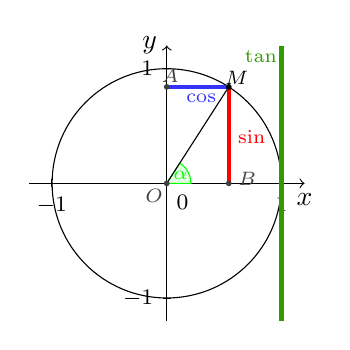
\begin{tikzpicture}[line join=round,x=2.0833333333333335cm,y=2.0833333333333335cm,scale=0.7]
      \draw[->,color=black] (-1.2,0) -- (1.2,0) node[below]{$x$};
      \foreach \x in {-1,1}
      \draw[shift={(\x,0)},color=black] (0pt,2pt) -- (0pt,-2pt) node[below] {\footnotesize $\x$};
      \draw[->,color=black] (0,-1.2) -- (0,1.2) node[left]{$y$};
      \foreach \y in {-1,1}
      \draw[shift={(0,\y)},color=black] (2pt,0pt) -- (-2pt,0pt) node[left] {\footnotesize $\y$};
      \draw[color=black] (0pt,-10pt) node[right] {\footnotesize $0$};
      \clip(-1.2,-1.2) rectangle (1.2,1.2);
      \draw [shift={(0,0)},color=qqwuqq,fill=qqwuqq,fill opacity=0.1] (0,0) -- (0:0.21) arc (0:57.13:0.21) -- cycle;
      \draw [line width=0.4pt] (0,0) circle (2.08cm);
      \draw (0,0)-- (0.54,0.84);
      \draw [line width=1.6pt,color=ttttff] (0,0.84)-- (0.54,0.84);
      \draw [line width=1.6pt,color=ffqqqq] (0.54,0.84)-- (0.54,0);
      \draw [line width=1.6pt,color=ttzzqq] (1,-1.2) -- (1,1.2);
      \begin{scriptsize}
        \fill [color=uququq] (0,0) circle (1.5pt);
        \draw[color=uququq] (-0.11,-0.11) node {$O$};
        \fill [color=black] (0.54,0.84) circle (1.5pt);
        \draw[color=black] (0.61,0.92) node {$M$};
        \fill [color=uququq] (0,0.84) circle (1.5pt);
        \draw[color=uququq] (0.03,0.94) node {$A$};
        \fill [color=uququq] (0.54,0) circle (1.5pt);
        \draw[color=uququq] (0.7,0.04) node {$B$};
        \draw[color=ttttff] (0.3,0.74) node {cos};
        \draw[color=ffqqqq] (0.74,0.4) node {sin};
        \draw[color=ttzzqq] (0.82,1.1) node {tan};
        \draw[color=qqwuqq] (0.12,0.07) node {$\alpha$};
      \end{scriptsize}
    \end{tikzpicture}
  \end{center}
  \end{minipage}
\end{Definition}\\
Es ergeben sich folgende (wissenswerte) Werte:
\\
\begin{center}
  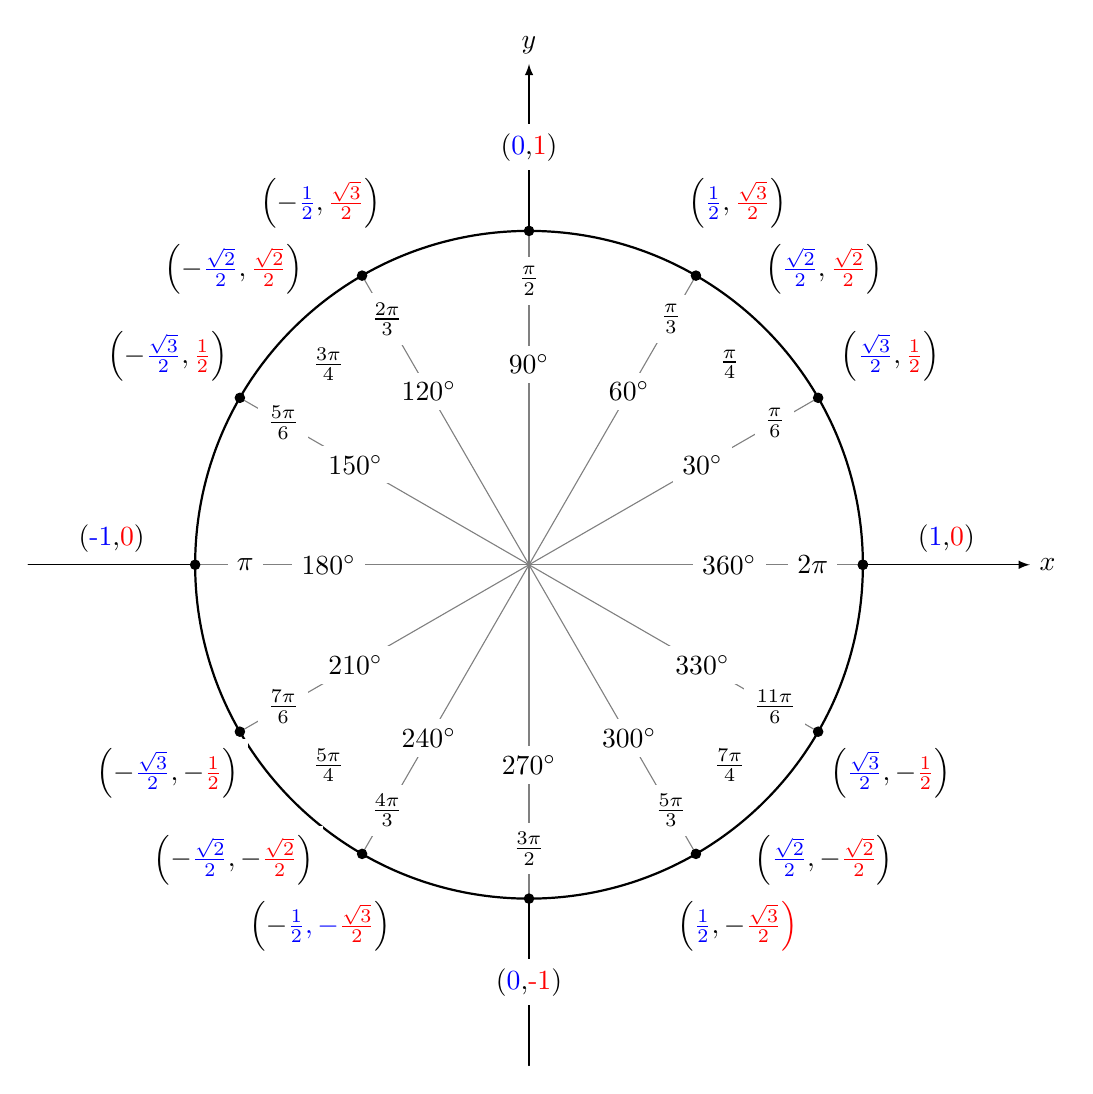
\begin{tikzpicture}[scale=5.3,cap=round,>=latex,scale=0.8]
    % draw the coordinates
    \draw[->] (-1.5cm,0cm) -- (1.5cm,0cm) node[right,fill=white] {$x$};
    \draw[->] (0cm,-1.5cm) -- (0cm,1.5cm) node[above,fill=white] {$y$};
    \draw[thick] (0cm,0cm) circle(1cm);
    \foreach \x in {0,30,...,360} {
            % lines from center to point
            \draw[gray] (0cm,0cm) -- (\x:1cm);
            % dots at each point
            \filldraw[black] (\x:1cm) circle(0.4pt);
            % draw each angle in degrees
            \draw (\x:0.6cm) node[fill=white] {$\x^\circ$};
    }
    \foreach \x/\xtext in {
        30/\frac{\pi}{6},
        45/\frac{\pi}{4},
        60/\frac{\pi}{3},
        90/\frac{\pi}{2},
        120/\frac{2\pi}{3},
        135/\frac{3\pi}{4},
        150/\frac{5\pi}{6},
        180/\pi,
        210/\frac{7\pi}{6},
        225/\frac{5\pi}{4},
        240/\frac{4\pi}{3},
        270/\frac{3\pi}{2},
        300/\frac{5\pi}{3},
        315/\frac{7\pi}{4},
        330/\frac{11\pi}{6},
        360/2\pi}
            \draw (\x:0.85cm) node[fill=white] {$\xtext$};

    \foreach \x/\xtext/\y in {
        30/\color{blue}\frac{\sqrt{3}}{2}\color{black}/\color{red}\frac{1}{2}\color{black},
        45/\color{blue}\frac{\sqrt{2}}{2}\color{black}/\color{red}\frac{\sqrt{2}}{2}\color{black},
        60/\color{blue}\frac{1}{2}\color{black}/\color{red}\frac{\sqrt{3}}{2}\color{black},
        150/-\color{blue}\frac{\sqrt{3}}{2}\color{black}/\color{red}\frac{1}{2}\color{black},
        135/-\color{blue}\frac{\sqrt{2}}{2}\color{black}/\color{red}\frac{\sqrt{2}}{2}\color{black},
        120/-\color{blue}\frac{1}{2}\color{black}/\color{red}\frac{\sqrt{3}}{2}\color{black},
        210/-\color{blue}\frac{\sqrt{3}}{2}\color{black}/-\color{red}\frac{1}{2}\color{black},
        225/-\color{blue}\frac{\sqrt{2}}{2}\color{black}/-\color{red}\frac{\sqrt{2}}{2}\color{black},
        240/-\color{blue}\frac{1}{2}/-\color{red}\frac{\sqrt{3}}{2}\color{black},
        330/\color{blue}\frac{\sqrt{3}}{2}\color{black}/-\color{red}\frac{1}{2}\color{black},
        315/\color{blue}\frac{\sqrt{2}}{2}\color{black}/-\color{red}\frac{\sqrt{2}}{2}\color{black},
        300/\color{blue}\frac{1}{2}\color{black}/-\color{red}\frac{\sqrt{3}}{2}}\color{black}
            \draw (\x:1.25cm) node[fill=white] {$\left(\xtext,\y\right)$};
    \draw (-1.25cm,0cm) node[above=1pt] {(\color{blue}-1\color{black},\color{red}0\color{black})}
          (1.25cm,0cm)  node[above=1pt] {(\color{blue}1\color{black},\color{red}0\color{black})}
          (0cm,-1.25cm) node[fill=white] {(\color{blue}0\color{black},\color{red}-1\color{black})}
          (0cm,1.25cm)  node[fill=white] {(\color{blue}0\color{black},\color{red}1\color{black})};
  \end{tikzpicture}
\end{center}
\\
Des Weiteren gilt:\\
\begin{center}
  \begin{tabu} to 0.9\textwidth{| X[c] | X[c] | X[c] | X[c] |}
    \hline
    & 15$^\circ$ & 45$^\circ$ & 75$^\circ$\\
    & $\dfrac{\pi}{12}$ & $\dfrac{\pi}{4}$ & $\dfrac{5\pi}{12}$\\
    \hline
    $\sin(\alpha)$ & $\dfrac{\sqrt{6}-\sqrt{2}}{4}$ & $\dfrac{1}{\sqrt{2}}$ & $\dfrac{\sqrt{6}+\sqrt{2}}{4}$\\
    \hline
    $\cos(\alpha)$ & $\dfrac{\sqrt{6}+\sqrt{2}}{4}$ & $\dfrac{\sqrt{3}}{2}$ & $\dfrac{\sqrt{6}-\sqrt{2}}{4}$\\
    \hline
  \end{tabu}
\end{center}

\section{Additions- und Verdopplungssätze}
\begin{Theorem}
    $$\cos(a - b)  = \cos(a)\cos(b) + \sin(a)\sin(b)$$
    $$\sin(a - b)  = \sin(a)\cos(b) - \cos(a)\sin(b)$$
    $$\cos(a + b)  = \cos(a)\cos(b) - \sin(a)\sin(b)$$
    $$\sin(a + b)  = \sin(a)\cos(b) + \cos(a)\sin(b)$$
\end{Theorem}
\begin{Bemerkung}
  Hieraus ergeben sich einige weitere Relationen, wie z.B. $\sin(2a)$. Diese lassen sich jedoch schnell und leicht herleiten.
\end{Bemerkung}
\section{Allgemeine Sinus- und Kosinussätze}
In einem beliebigen Dreieck gelten abgewandelte Formen der aus der 8. Klasse bekannten Sätze:
\begin{Theorem}
  \begin{minipage}{0.6\textwidth}
    \begin{itemize}
      \item $\dfrac {a} {sin(\alpha)}=\dfrac {b} {sin(\beta)}=\dfrac {c} {sin(\gamma)}$
      \item $c^2=a^2+b^2-2abcos(\gamma)$
    \end{itemize}
  \end{minipage}
  \begin{minipage}{0.4\textwidth}
    \definecolor{qqwuqq}{rgb}{0,50,0}
    \begin{tikzpicture}[line cap=round,line join=round,>=triangle 45,x=0.5cm,y=0.6cm]
      \clip(-0.4,-4.3) rectangle (9,3);
      \draw [shift={(4.22,1.92)},color=qqwuqq,fill=qqwuqq,fill opacity=0.5] (0,0) -- (-134.14:1.5) arc (-134.14:-47.61:1.5) -- cycle;
      \draw [shift={(-0.38,-2.82)},color=qqwuqq,fill=qqwuqq,fill opacity=0.5] (0,0) -- (1.04:1.5) arc (1.04:45.86:1.5) -- cycle;
      \draw [shift={(8.4,-2.66)},color=qqwuqq,fill=qqwuqq,fill opacity=0.5] (0,0) -- (132.39:1.5) arc (132.39:181.04:1.5) -- cycle;
      \draw (4.22,1.92)-- (8.4,-2.66);
      \draw (4.22,1.92)-- (-0.38,-2.82);
      \draw (8.4,-2.66)-- (-0.38,-2.82);
      \begin{scriptsize}
        \draw[color=black] (6.7,-0.44) node {$a$};
        \draw[color=black] (1.76,-0.08) node {$b$};
        \draw[color=black] (4.06,-2.28) node {$c$};
        \draw[color=black] (4.4,1.05) node {$\gamma$};
        \draw[color=black] (0.7,-2.45) node {$\alpha$};
        \draw[color=black] (7.5,-2.2) node {$\beta$};
      \end{scriptsize}
    \end{tikzpicture}
  \end{minipage}
\end{Theorem}
\begin{Bemerkung}
  Man bemerkt, dass sich die bekannten Relationen ergeben, wenn einer der Winkel den Wert $\dfrac{\pi}{2}$ annimmt.
\end{Bemerkung}
\section{Sinusfunktionen}
Zur Vollständigen Funktionsdiskussion einer Sinus-Funktion sind einige Besonderheiten zu beachten:
\begin{enumerate}
  \item Amplitude und Periodizität\\
  Eine Funktion der Form $f(x)=a\cdot\sin(b(x-c))+d$ hat:
  \begin{itemize}
    \item die Periode $P = \dfrac{2\pi}{|b|}$
    \item die Amplitude $A = |a|$
    \item die Verschiebung entlang der $x$-Achse um $d$ und entlang der $y$-Achse um $c$
    \end{itemize}
  \item Symmetrieeigenschaften\\
  Hier sollte zumindest bekannt sein, dass $f(x)=\sin(x)$ punktsymmetrisch zum Origo ist, und dass $f(x)=\cos(x)$ Achsensymmetrisch zur $y$-Achse ist.
  \item Die Null-, Extrem- und Wendestellen sind in Form einer Menge anzugeben. (Es sei denn, die Aufgabenvorschrift fordert explizit zu einer Begrenzung auf ein angegebenes Intervall auf)\\
  \begin{Beispiel}
    Die Nullstellen der Funktion $f(x)=\sin(x)$ lassen sich dartstellen als: $x \in \{k\pi|k \in \Z\}$
  \end{Beispiel}
  \item Bei der Teilung durch eine Sinusfunktion können Definitionslücken an dessen Nullstellen entstehen. Auch diese können in der bereits gezeigten Form angegeben werden.
  \end{enumerate}
\subsection{Zusammengesetzte Sinusfunktionen}
\section{Polarkoordinaten}
In der Kursstufe beschränken wir uns auf die Benutzung von Polarkoordinaten für Punkte in der Ebene (2D).
\begin{Definition}
  Polarkoordinaten sind eine Form der eindeutigen Punktangaben, doch anstatt wie kartesische Koordinaten 2 Entfernungen $x$ und $y$ zu verwenden, haben sie die Form $(r|\varphi)$. $r$ ist hierbei die Entfernung zum Origo und $\varphi$ ein orientierter Winkel (in $rad$).
\end{Definition}

\subsection{Umrechnung}
\begin{minipage}{0.5\linewidth}
\textbf{Kartesisch $\rightarrow$ Polar}
\begin{itemize}
  \item  $r=\sqrt{x^2+y^2}$
  \item $\varphi = \tan(\dfrac{y}{x})$
\end{itemize}
\textbf{Polar $\rightarrow$ Kartesisch}
\begin{itemize}
  \item $x = r\cdot\cos(\varphi)$
  \item  $y=r\cdot\sin(\varphi)$
\end{itemize}
\end{minipage}
\begin{minipage}{0.5\linewidth}
  \definecolor{zzzzzz}{rgb}{0.6,0.6,0.6}
  \definecolor{ffqqqq}{rgb}{1,0,0}
  \definecolor{qqzztt}{rgb}{0,0.6,0.2}
  \definecolor{qqqqff}{rgb}{0,0,1}
  \begin{tikzpicture}[line cap=round,line join=round,>=triangle 45,x=2.0cm,y=2.0cm]
    \draw[->,color=black] (-0.31,0) -- (3.05,0);
    \foreach \x in {,0.5,1,1.5,2,2.5,3}
    \draw[shift={(\x,0)},color=black] (0pt,-2pt);
    \draw[color=black] (2.9,0.02) node [anchor=south west] {$x$};
    \draw[->,color=black] (0,-0.5) -- (0,2.19);
    \foreach \y in {-0.5,0.5,1,1.5,2}
    \draw[color=black] (0.03,2.1) node [anchor=west] {$y$};
    \clip(-0.31,-0.5) rectangle (3.05,2.19);
    \draw [shift={(0,0)},line width=1.6pt,color=ffqqqq,fill=ffqqqq,fill opacity=0.1] (0,0) -- (0:0.53) arc (0:42.19:0.53) -- cycle;
    \draw [line width=1.6pt,color=qqzztt] (0,0)-- (2.14,1.94);
    \draw [line width=1.6pt,color=zzzzzz] (0,1.94)-- (2.14,1.94);
    \draw [line width=2pt,color=zzzzzz] (2.14,1.94)-- (2.14,0);
    \begin{scriptsize}
      \fill [color=qqqqff] (2.14,1.94) circle (1.7pt);
      \draw[color=qqqqff] (2.19,2.02) node {$P$};
      \draw[color=qqzztt] (1.15,0.94) node {$r$};
      \draw[color=ffqqqq] (0.36,0.17) node {$\varphi$};
      \draw[color=zzzzzz] (1.11,1.89) node {$x$};
      \draw[color=zzzzzz] (2.25,0.94) node {$y$};
    \end{scriptsize}
  \end{tikzpicture}
\end{minipage}



\section{Beispiele einer Funktionsdiskussion}

\subsection{$f(x)=2\cos(x)+2\sin(x)\cos(x)$}
Sei die Funktion $f(x)=2\cos(x)+2\sin(x)\cos(x)$, ihr Schaubild sei K.\\
Untersuchen Sie K im Intervall $[0;2\pi]$ auf gemeinsame Punkte mit der $x$-Achse, sowie Extrem- und Wendepunkte. Zeichnen Sie K im Intervall $[0;2\pi]$. Untersuchen Sie K auf Symmetrie.
\\\\
\begin{tabular}{ p{0.5\textwidth} | p{0.5\textwidth} }
  \textbf{Definitionsmenge}  & \textbf{Periodizität und Amplitude}                                                   \\
  $D = \R$                  & Die Periode von $f$ ist $P=2\pi$. Die Amplitude $A$ beträgt $\dfrac{3}{2}\sqrt{3}$.   \\
\end{tabular}
\\

\begin{minipage}[t]{0.5\textwidth}
  \textbf{Nullstellen}\\
  \underline{Notwendige und hinreichende Bedingung:}\\
  \begin{align*}
    f(x)                                        &=0\\
    \Leftrightarrow 2\cos(x)+2\sin(x)\cos(x)    &=0\\
    \Leftrightarrow 2\cos(x)(1+\sin(x))         &=0\\
    \stackrel{S.d.N}{\Rightarrow}
    \left\{\begin{array}{rccl}
      2\cos(x)  &=  &0  & \\
      1+\sin(x) &=  &0  &
    \end{array} \\
    \Leftrightarrow
    \left\{ \begin{array}{rccl}
      \cos(x) & = & 0 \\
      \sin(x) & = & -1
    \end{array} \\
    \Leftrightarrow
    \left\{ \begin{array}{rccl}
      x_1&=&\dfrac{1}{2}\pi&  \\\\
      x_2&=&\dfrac{3}{2}\pi&
    \end{array} \\
    \Rightarrow \mathbb{L} &= \left \{ \left( \dfrac{1}{2} \pi \middle| 0 \right) ; \left( \dfrac{3}{2} \pi \middle| 0 \right) \right\}
  \end{align*}
\end{minipage}
\vline
\begin{minipage}[t]{0.5\textwidth}
  \textbf{Ableitungen}\\
    \begin{align*}
      f'(x)&=-2\sin(x)+2(\cos(x)\cos(x)-\sin(x)\sin(x))\\
      &=-2\sin(x)+2(\cos^2(x)-\sin^2(x))\\
      &=-2\sin(x)+2(1-\sin^2(x)-\sin^2(x))\\
      &=-4\sin^2(x)-2\sin(x)+2\\
      f''(x)&=-4(\cos(x)\sin(x)+\sin(x)\cos(x))-2\cos(x)\\
      &=-8\sin(x)\cos(x)-2\cos(x)\\
      f'''(x)&=-8(\cos(x)\cos(x)-\sin(x)\sin(x))+2\sin(x)\\
      &=-8(1-\sin^2(x)-\sin^2(x))+2\sin(x)\\
      &=16\sin^2(x)+2\sin(x)-8
    \end{align*}#
\end{minipage}
\\\\

\textbf{Extremstellen}\\

\begin{minipage}[t]{0.5\textwidth}
  \underline{Notwendige Bedingung:}\\
    $f'(x)&=0$\\
    $\Leftrightarrow4\sin^2(x)-2\sin(x)+2&=0$\\
    Substitution: $y&=\sin(x)$\\
    $\Rightarrow4y^2-2y+2=0$\\
    $\stackrel{ABC-Formel}{\Rightarrow}y_{1,2}=\dfrac{2\pm\sqrt{(-2)^2-4*(-4)*2}}{-8}$\\
    Resubsitution:\\
    $\Rightarrow
    \left\{\begin{array}{rccl}
      \sin(x)&=\dfrac{2+\sqrt{20}}{-8}\\
      \sin(x)&=\dfrac{2-\sqrt{20}}{-8}
    \end{array}\right\\
    \Rightarrow\mathbb{L}=\left\{\dfrac{1}{6}\pi;\dfrac{5}{6}\pi;\dfrac{3}{2}\pi\right\}$
\end{minipage}
\vline
\begin{minipage}[t]{0.5\textwidth}
  \underline{Hinreichende Bedingung:}\\
    $f''(x)&\neq0$\\
    \Rightarrow
    \left\{\begin{array}{rccl}
      f''\left(\dfrac{1}{6}\pi\right)&\stackrel{?}{=}0\\\\
      f''\left(\dfrac{5}{6}\pi\right)&\stackrel{?}{=}0\\\\
      f''\left(\dfrac{3}{2}\pi\right)&\stackrel{?}{=}0
    \end{array}\right\\
    \Leftrightarrow
    \left\{\begin{array}{rccl}
      8\sin\left(\dfrac{1}{6}\pi\right)\cos\left(\dfrac{1}{6}\pi\right)-2\sin\left(\dfrac{1}{6}\pi\right)&\stackrel{?}{=}0\\\\
      8\sin\left(\dfrac{5}{6}\pi\right)\cos\left(\dfrac{5}{6}\pi\right)-2\sin\left(\dfrac{5}{6}\pi\right)&\stackrel{?}{=}0\\\\
      8\sin\left(\dfrac{3}{2}\pi\right)\cos\left(\dfrac{3}{2}\pi\right)-2\sin\left(\dfrac{3}{2}\pi\right)&\stackrel{?}{=}0
    \end{array}\right\\
    \Leftrightarrow
    \left\{\begin{array}{rccl}
      8*\dfrac{1}{2}*\dfrac{\sqrt{3}}{2}-2*\dfrac{\sqrt{3}}{2}&\stackrel{!}{\neq}&0&,  <0 \Rightarrow HP\\
      8*\dfrac{1}{2}*-\dfrac{\sqrt{3}}{2}-2*-\dfrac{\sqrt{3}}{2}&\stackrel{!}{\neq}&0&,  >0 \Rightarrow TP\\
      8*(-1)(0)-2(0)&\stackrel{!}{=}&0& \Rightarrow \text{kein } EP
    \end{array}\right\\
\end{minipage}
\underline{Ergebnis}\\
Auf dem Intervall $[0;2\pi]$  besitzt K den Hochpunkt H$\left(\dfrac{1}{6}\pi|f\left(\dfrac{1}{6}\pi\right)\right)$ und den Tiefpunk T$\left(\dfrac{5}{6}\pi|f\left(\dfrac{5}{6}\pi\right)\right)$.\\
$\Leftrightarrow$ H$\left(\dfrac{1}{6}\pi|\dfrac{3}{2}\sqrt{3}\right)$ und T$\left(\dfrac{5}{6}\pi|-\dfrac{3}{2}\sqrt{3}\right)$.
\\\\

\textbf{Wendestellen}\\

\begin{minipage}[t]{0.5\textwidth}
  \underline{Notwendige Bedingung:}\\
  \begin{align*}
    f''(x)=0\\
    \Leftrightarrow -8\sin(x)\cos(x)-2\cos(x)=0\\
    \Leftrightarrow \cos(x)(-2-8\sin(x))=0\\
    \stackrel{SdN}{\Rightarrow}
    \left\{\begin{array}{rccl}
      \cos(x)&=&0\\
      \sin(x)&=&-\dfrac{1}{4}
    \end{array}\right\\
    \Rightarrow \mathbb{L}=\left\{\dfrac{1}{2}\pi;\dfrac{3}{2}\pi;\sim3,394;\sim6,031\right\}
  \end{align*}
\end{minipage}
\vline
\begin{minipage}[t]{0.5\textwidth}
  \underline{Hinreichende Bedingung:}\\
    $f'''(x)&\neq0$\\
    \Rightarrow
    \left\{\begin{array}{rccl}
      f'''\left(\dfrac{1}{2}\pi\right)&\stackrel{?}{=}0\\\\
      f'''\left(\dfrac{3}{2}\pi\right)&\stackrel{?}{=}0\\\\
      f'''\left(3,394)&\stackrel{?}{=}0\\\\
      f'''\left(6,031)&\stackrel{?}{=}0
    \end{array}\right\\
    \Leftrightarrow
    \left\{\begin{array}{rccl}
      16\sin^2\left(\dfrac{1}{2}\pi\right)+\sin\left(\dfrac{1}{2}\pi\right)-8&\stackrel{?}{=}0\\\\
      16\sin^2\left(\dfrac{3}{2}\pi\right)+\sin\left(\dfrac{3}{2}\pi\right)-8&\stackrel{?}{=}0\\
      16\sin^2(3,394)+\sin(3,394)-8&\stackrel{?}{=}0\\
      16\sin^2(6,031)+\sin(6,031)-8&\stackrel{?}{=}0
    \end{array}\right\\
    \Leftrightarrow
    \left\{\begin{array}{rccl}
      16*1+1-8&\stackrel{!}{\neq}&0&,>0\Rightarrow WP\\
      16*1-1-8&\stackrel{!}{\neq}&0&,>0\Rightarrow WP\\
      -7,5&\stackrel{!}{=}&0&,<0\Rightarrow WP\\
      -7,5&\stackrel{!}{=}&0&,<0\Rightarrow WP&
    \end{array}\right\\
\end{minipage}
\begin{Bemerkung}
  Außerdem: $f'\left(\dfrac{3}{2}\pi\right)=0\Rightarrow$ Sattelpunkt
\end{Bemerkung}

\underline{Ergebnis}\\
Auf dem Intervall $[0;2\pi]$  besitzt K die Wendepunkte $\left(\dfrac{1}{2}\pi\middle|f\left(\dfrac{1}{2}\pi\right)\right)$, $(3,394|f(3,394))$, $(6,031|f(6,031))$ und den Sattelpunkt $\left(\dfrac{3}{2}\pi\middle|f\left(\dfrac{3}{2}\pi\right)\right)$.\\
\Leftrightarrow $W_1\left(\dfrac{1}{2}\pi\middle|0\right)$, $W_2(3,394|-1,452)$, $W_3(6,031|1,452)$, $S\left(\dfrac{3}{2}\pi\middle|0\right)$.\\
\\\\

\textbf{Schaubild}\\

\definecolor{ccqqqq}{rgb}{0.8,0,0}
\definecolor{cqcqcq}{rgb}{0.75,0.75,0.75}
\begin{tikzpicture}[line cap=round,line join=round,>=triangle 45,x=1.0cm,y=1.0cm]
  \draw [color=cqcqcq,dash pattern=on 1pt off 1pt, xstep=1.0cm,ystep=1.0cm] (-0.62,-3.28) grid (7.22,3.26);
  \draw[->,color=black] (-0.62,0) -- (7.22,0);
  \foreach \x in {,1,2,3,4,5,6,7}
  \draw[shift={(\x,0)},color=black] (0pt,-2pt) node[below] {\footnotesize $\x$};
  \draw[color=black] (7.04,0.04) node [anchor=south west] { x};
  \draw[->,color=black] (0,-3.28) -- (0,3.26);
  \foreach \y in {-3,-2,-1,1,2,3}
  \draw[shift={(0,\y)},color=black] (2pt,0pt) -- (-2pt,0pt) node[left] {\footnotesize $\y$};
  \draw[color=black] (0.05,3.05) node [anchor=west] { y};
  \draw[color=black] (0pt,-10pt) node[right] {\footnotesize $0$};
  \draw[color=ccqqqq] (1.5,2.5) node {K};
  \clip(-0.62,-3.28) rectangle (7.22,3.26);
  \draw[line width=1.6pt,color=ccqqqq, smooth,samples=100,domain=-0.6249016652708163:7.217846281536262] plot(\x,{2*cos(((\x))*180/pi)+2*sin(((\x))*180/pi)*cos(((\x))*180/pi)});
\end{tikzpicture}
\\\\

\textbf{Symmetrie}\\

K ist punktsymmetrisch zu $W_1$, denn es gilt:
\begin{align*}
  f(\dfrac{1}{2}\pi+x)&=-1*f(\dfrac{1}{2}\pi-x)\\
  \Leftrightarrow
  2\cos(\dfrac{1}{2}\pi+x)+2\sin(\dfrac{1}{2}\pi+x)\cos(\dfrac{1}{2}\pi+x)&=-1*(2\cos(\dfrac{1}{2}\pi-x)+2\sin(\dfrac{1}{2}\pi-x)\cos(\dfrac{1}{2}\pi-x))\\
  \Leftrightarrow
  -2\sin(x)-2\cos(x)\sin(x)&=-1*(2\sin(x)+2\cos(x)\sin(x))
\end{align*}
K ist außerdem zu $S$ punktsymmetrisch, denn es gilt:
\begin{align*}
  f(\dfrac{3}{2}\pi+x)&=-1*f(\dfrac{3}{2}\pi-x)\\
  \Leftrightarrow
  2\cos(\dfrac{3}{2}\pi+x)+2\sin(\dfrac{3}{2}\pi+x)\cos(\dfrac{3}{2}\pi+x)&=-1*(2\cos(\dfrac{3}{2}\pi-x)+2\sin(\dfrac{3}{2}\pi-x)\cos(\dfrac{3}{2}\pi-x))\\
  \Leftrightarrow
  2\sin(x)+2\cos(x)\sin(x)&=-1*(-2\sin(x)-2\cos(x)\sin(x))
\end{align*}
